现代 ECG 深度模型在同分布(ID)下取得出色的准确率和校准性能，但其在分布偏移下的可靠性仍是部署的核心开放问题\cite{ovadia2019calibration,guo2017calibration,wagner2020ptbxl}。重校准方法在带标签的校准划分上拟合少量参数或一个灵活映射；其效益——期望校准误差(Expected Calibration Error, ECE)的降低——在同一分布上度量。当模型部署到偏移目标时，该效益会衰减或反转。

\textbf{该问题对 ECG 的重要性。} PTB-XL \cite{wagner2020ptbxl}、Chapman-Shaoxing \cite{zheng2022ecgarrhythmia} 和 CPSC 呈现出实质上不同的采集协议、导联集和标签词表。在一个机构数据上训练并校准的模型，在下一个机构会遭遇协变量、先验概率和标签概念偏移\cite{morenotorres2012}。临床医生和监管者需要一条决策规则：\emph{在我本地数据预算和我可度量的偏移给定下，我应部署重校准模型、购买标签并重校准，还是拒绝部署？}

\textbf{温度缩放：ID vs.\ OOD 的经验期望。} 温度缩放(TS)是一种单调的事后 softmax 温度变换\cite{guo2017calibration}。在凸损失下于带标签的校准划分上拟合时，TS 在该处最小化 NLL；在同一分布上其校准效益在经验上较小，而在偏移目标上，源拟合温度与目标 logit 分布失配，可保留非平凡的校准效益。我们强调这种不对称性是\emph{经验性的}，而非定理：ECE 在置信度平移的单调映射下并非不变，且当模型在目标上欠置信时，TS 可能\emph{增加} ECE(我们自己的数据包含九个此类显著负单元)。这种 ID 与 OOD 的不对称性促使我们采用预注册的主要终点 $\Delta\text{ECE}_{\text{OOD}}$，而非原计划的衰减量 $\Delta\text{ECE}_{\text{OOD}}-\Delta\text{ECE}_{\text{ID}}$(修订 A1，见 Sec.~\ref{sec:prereg})。

\textbf{预注册 + 多种子验证设计。} 为避免 HARKing(在结果已知后形成假设，Hypothesis After Results Known)，我们在多种子验证揭盲前预注册协议 v2.1-A1 \cite{protocolv21a1}，包含书面主要终点、主检验、族结构和失败分支。修订 A1 将主要终点从 \texttt{decay} 重新定位到 $\Delta\text{ECE}_{\text{OOD}}$，由与经验不对称性一致的一次独立探索性预实验触发；该修订作为预注册修订归档\cite{nosek2019prereg,lakens2019prereg}，附带修订前后的协议哈希。多种子验证(5 种子 $\times$ 6 迁移对 $\times$ 2 架构)提供鲁棒性证据；全部 60 个种子结果，包括九个反例，均透明报告。

\textbf{贡献。} 我们做出五项独立贡献：
\begin{description}
    \item[\textbf{C1} (主要，OOD 效益量化)：] 在预注册的主要终点 $\Delta\text{ECE}_{\text{OOD}}$ 上，TS 在跨 6 迁移对 $\times$ 2 架构的 51/60 种子实验中产生统计显著的正向 OOD 校准效益(InceptionTime 27/30，ResNet1D 24/30)，九个反例透明披露并给予机理解释。六个 InceptionTime 方向中有三个达到 5/5 完全支持；其余三个达到 4/5，各有一个反例。六个 ResNet1D 方向中有两个达到 5/5 完全支持；两个达到 4/5；两个达到 3/5。
    \item[\textbf{C2} (边界条件，预注册分支触发)：] 在全部 12 个对$\times$架构分层中，23/60 单元(38.3\%；BCa operating CI)的 95\% CI 包含零，34/60 的 CI 下界 $>0$(分层均值范围 $-0.0008$ 至 $+0.0232$；总体 ID 均值 $+0.0083$ vs.\ OOD 均值 $+0.0159$)。预注册的边界判据(CI 包含零的单元 $\geq$80\%)\emph{未}满足，因此触发预注册的``ID 非零边界''分支(协议 A1.4.2)：重新审视``TS 不存在 ID 可重校准的误校准''这一前提，衰减对比终点作为探索性恢复，C1 据此加以限定——OOD 效益平均约为 ID 效益的 $1.9\times$，但\emph{不能}完全归因于 OOD 特有的失配。$47/60 = 78.3\%$ 的 ID 点估计为正，$2/60 = 3.3\%$ 满足 $\Delta\text{ECE}_{\text{ID}} < -0.01$：过校正情形(反例 6，$-0.0152$)和一个边缘情形($-0.0128$)。
    \item[\textbf{C3} (方法学，Shapley 分解验证)：] 27 单元全因子合成验证(斜率$\times$截距$\times$患病率，$n=20{,}000$)在很大程度上证实：斜率/截距/患病率分解在可辨识区间内恢复真值($n=20{,}000$ 时 27/27 通过；$n=500$ 时 21/27)，并在无阈值情况下标记纠缠区域，对绝对 Shapley 值给出自助 CI。
    \item[\textbf{C4} (实用，方法选择边界)：] 在 8 重校准方法 $\times$ 6 迁移对 $\times$ 5 种子 $\times$ 2 架构上，TS 鲁棒(51/60 支持)，而 EM 先验适配在包含病态单元($w_{\text{ID}}>10$)时脆弱(InceptionTime 15/30 支持)；排除这些单元后 EM 的 OOD 发现衰减。其机制为先验-似然失配：当源估计的混淆矩阵病态时，EM 拟合的目标先验放大而非校正由偏移引起的误校准。
    \item[\textbf{C5} (临床，判别感知校准门)：] 两层部署门将校准有效性(C1：$\Delta\text{ECE}_{\text{OOD}}>0$)与临床可行性(准确率 $\geq$ 源域基线)解耦。在 14 个对$\times$架构分层中，7/14 同时通过两层，可部署；7/14 未通过判别层，被正确拒绝——包括 $\Delta\text{ECE}_{\text{OOD}}$ 为正但准确率低于源基线的方向(例如 PTB-XL$\rightarrow$Chapman ResNet1D：$\Delta\text{ECE}=+0.029$ 但 $\text{acc}=0.657 < 0.713$)。该门将 9/60 反例重构：4/9 为校准失败(C1 拒绝)，5/9 为判别失败(C1 通过但 C5 拒绝)，提供将校准有效性与临床可行性分离的两层部署判据。
\end{description}

这一框架填补了一项空白：先前的 ECG 校准研究报告了该现象\cite{barandas2023,zhang2022,physiolmeas2026,medrxiv2026}，但未给出具有多种子鲁棒性证据的可操作``\emph{TS 何时获益}''答案。本文的新意\emph{并非}``在 ECG 上做多种子验证''(多种子验证是方法学选择，而非科学贡献)；新意在于\textbf{首次系统刻画跨语料库 ECG 迁移中 TS 产生正向 OOD 校准效益的边界条件}，包括 (i) 以预注册终点和多种子鲁棒性证据进行 OOD 效益量化，(ii) 触发预注册分支的 ID 边界条件分析(BCa operating CI 下 38.3\% CI 包含零的单元，$<$ 80\%)，(iii) 方法选择边界(TS 鲁棒 vs.\ EM 先验和矩阵缩放最弱)，(iv) 诚实报告可预测性失败分支，(v) 将校准有效性与临床可部署性解耦的判别感知校准门。这一边界条件刻画是可操作的贡献；多种子验证是施加于每个边界的证据标准。

\begin{figure}[htbp]
\centering
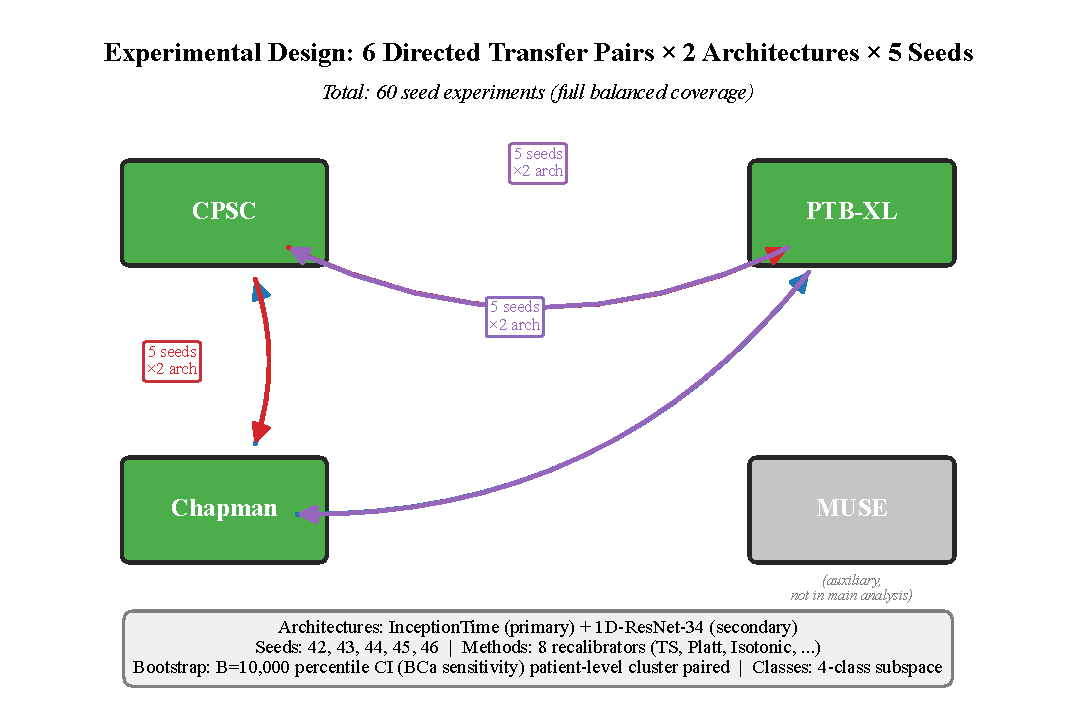
\includegraphics[width=0.95\columnwidth]{figures/fig_design_overview.pdf}
\caption{实验设计概览。三个 ECG 语料库(CPSC、Chapman、PTB-XL)之间的六个有向跨语料库迁移对，每对在两种架构(InceptionTime、1D-ResNet-34) $\times$ 5 种子(42--46)上评估，产生 60 个完全平衡的种子实验。MUSE 作为辅助语料库显示，不进入主分析。每对以 8 种重校准方法和患者层级聚类配对自助法($B=10{,}000$，BCa operating CI)评估。}
\label{fig:design_overview}
\end{figure}
